\chapter{Diseño}
\label{cap:disenio}

En esta sección se especificarán los aspectos más relevantes para el desarrollo del sistema: tecnologías a utilizar, cómo y por qué utilizarlas, etc. A continuación se profundizará en las herramientas a utilizar en cada una de las partes de la plataforma web y, para una mejor comprensión, dividiremos este apartado en tres: servidor (\textit{backend}), cliente (\textit{frontend}) e infraestructura.

\section{Backend}

\subsection{Patrón Modelo-Vista-Controlador}

Para el desarrollo se plantea basarse en el patrón de arquitectura software Modelo-Vista-Controlador (MVC), cuyos principios se basan en separar los datos y la lógica de la aplicación de su interfaz, con el objetivo de facilitar el desarrollo y mantenimiento de la aplicación. De este modo, distinguimos los siguientes componentes:

\begin{itemize}
    \item \textbf{Modelo}: representa la información con la que opera el sistema. Gestiona los accesos a dicha información, como consultas y actualizaciones. Se encarga de enviar a la vista la información que solicite para su visualización. Las peticiones de acceso a dicha información llegan a éste a través del controlador.
    \item \textbf{Vista}: presenta el modelo en el formato adecuado. En este caso, la vista es el \textit{frontend} de nuestra aplicación.
    \item \textbf{Controlador}: responde a los eventos, invoca peticiones al modelo para solicitar información y puede enviar comandos a su vista asociada.
\end{itemize}

Una vez presentado el patrón, debemos buscar una tecnología que se adapte a este. Finalmente, nos decantaremos por Django, un framework de alto nivel para trabajar con python en el servidor.

\subsection{Django} \cite{Dj}
Como decíamos, Django se trata de un framework de desarrollo web a alto nivel y de código abierto (licencia BSD), escrito en Python y que representa el patrón de diseño Modelo-vista-controlador. Su meta fundamental es facilitar la creación de sitios web complejos, haciéndo énfasis en la reutilización, conectividad y extensibilidad de componentes, el desarrollo ágil y el principio No te repitas (DRY, del inglés \textit{Don't Repeat Yourself}). A continuación se exponen algunas de las razones por las que elegir a Django frente a otros frameworks de desarrollo web.

\begin{itemize}
    \item ORM: se trata de una potente herramienta de base de datos. Basándose en los modelos que el usuario codifique, Django es capaz de convertirlos a una base de datos orientada a objetos. Además, se ofrece soporte a diversos Sistemas Gestores de Base de Datos (MySQL, MariaDB, PostgreSQL, Oracle y SQLite), unificados bajo una misma sintaxis y dejando de lado a SQL como lenguaje de consultas.
    \item Formularios: Gracias a Django la validación de formularios es mucho más sencilla. Solamente tienes que definir los atributos de tus modelos y como quieres que funcione la validación básica.
    \item Panel de administración: Django ofrece un panel de administración altamente personalizable que puede incluso utilizarse como area de administración final en tu aplicación web.
    \item Django no es PHP: para aquellos que busquen un cambio, Django es una gran alternativa a PHP, además de tener una gran comunidad de usuarios detrás.
    \item Django es Python, un lenguaje de scripting elegante y potente con una gran comunidad de usuarios detrás.
    \item Proyectos existosos construidos en Django \cite{SUDj}: 
    \begin{itemize}
        \item Disqus \cite{Disqus}: plataforma que ofrece un sistema de discusiones para tu blog o sitio web.
        \item Instagram \cite{Instagram}: la aplicación más famosa para subir imágenes y aplicar efectos en ellas.
        \item Open Stack \cite{Open Stack}: proyecto de computación en la nube que proporciona una Infraestructura Como Servicio (IaaS).
        \item Pinterest \cite{Pinterest}: red social para compartir imágenes que permite a los usuarios crear y administrar en tableros personales temáticos colecciones de imágenes, como eventos, intereses o aficiones entre otros.
    \end{itemize}
\end{itemize}

\subsubsection{Modelo-Template-Vista}
Un aspecto a tener en cuenta en Django, es que no representa el patrón Modelo-vista-controlador como tal, si no que se basa en lo que podríamos denominar ``Modelo-template-vista''. Si bien es cierto que se asemeja mucho a la implementación del patrón MVC, para Django la Vista describe ``qué'' datos serán presentados y no ``cómo'' se verán los mismos, siéndo los \textit{templates} los encargados de esta última tarea.

Esto se debió a que los desarrolladores del framework no buscaron apegarse a nada en particular, sino desarrollar una herramienta que funcionara lo mejor posible.

\begin{figure}[H]
  \begin{center}
  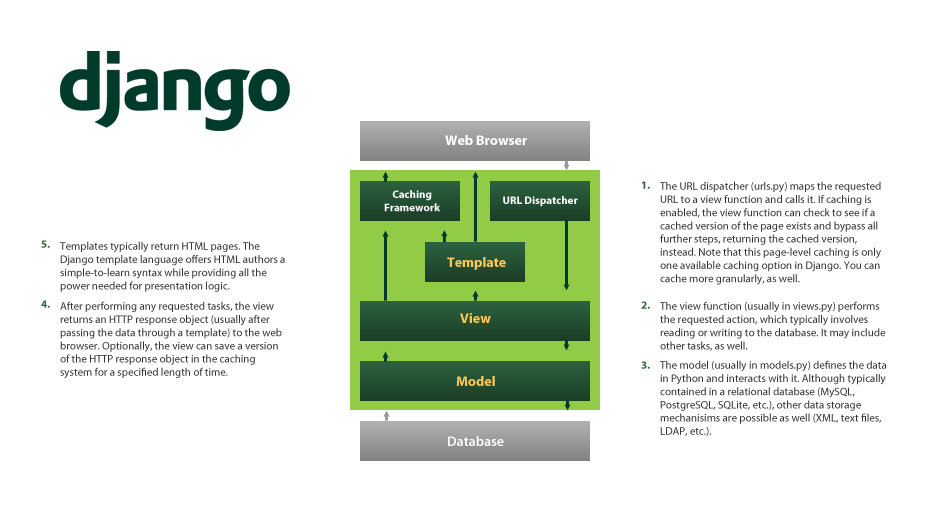
\includegraphics[width=0.8\textwidth]{../images/django_arch.png}
  \caption{Arquitectura de Django}
  \label{fig:django_arch}
  \end{center}
\end{figure}

\subsubsection{Sistema Gestor de Base de Datos}
El Sistema Gestor de Base de Datos es el encargado de proporcionar la capa de acceso a la información de la base de datos. Como hemos comentado, haciendo uso del ORM de Django, utilizaremos un conector para base de datos SQLite durante el desarrollo, que se modificará por un MySQL o postgreSQL para las fases de ``puesta en marcha'' (\textit{staging}) y producción.

\section{Frontend}
El \textit{frontend} es la capa de presentación de la aplicación, encargada de maquetar la estructura semántica del contenido (HTML), codificar el diseño en hojas de estilo (CSS) y agregar la interacción con el usuario (Javascript). En este proyecto, el cliente representará un papel bastante importante con respecto a la experiencia del usuario en la plataforma. Por ello, se trabajará además con una librería de Javascript, jQuery, que nos ayudará a dicho propósito, facilitando algunas tareas. 

\subsection{jQuery y Ajax}
Como comentantamos, jQuery \cite{jQuery} es una librería de Javascript, que facilita la interacción con los documentos HTML mediante la manipulación del árbol DOM.

\subsection{Bootstrap}

\section{Infraestructura}

\subsection{Github}

\subsection{Travis-CI}

\subsection{Plataforma Como Servicio}

\subsubsection{Openshift}

\subsection{Provisionamiento: Ansible}

\subsection{Ejecución automática de comandos en remoto. Fabric}

